\chapter{Fur: An Intelligent Fault Tolerance System}
\label{c:fur}

This chapter describes how subsystems in Fur collaborate to provide fault tolerance
for applications. First we will describe how users could specify fault
tolerance policy for the application, and then how WuKong Master take
the policy, application and discovery results and compile into low-level
intermediate representation that could be deployed to the network. Lastly, we 
describe how the sensor network detect, recognize, and recover from failures
autonomously based on the result of the mapping.

\section{WuKong Applications}

~\ref{application} illustrates a typical WuKong application with components
connecting to form a small network. What this figure shows is that applications
are made of components, and components are connected through properties.
Any pair of properties form links that binds components together. Connected
components interact with each other based on the direction of the connection.
The properties on the left of a component are inputs to this component, to the
right side are the outputs of an component. Thus one can infer that
a connection cannot connect to both inputs or outputs of any pair of components
as both of them have the same data flow.

\section{Fault Tolerance Policy}

In this work, fault tolerance policy can only be specified on the level of
components, so there is a separate policy for every component. For every
compoennt, users can specify two rules to guide and influence how fault
tolerance works at the hardware level.

Of all policy parameters to model a fault tolerant system, there are two that
are required for any fault tolerance systems in environment unique to WuKong.

\begin{enumerate}
\item \emph{Minimum Redundancy Level} The minimum number of devices that will be
supported as a backup for a particular component. Therefore when one of the
devices fail, others will take over.

\item \emph{Maximum Reaction Time} The maximum latency a failure will take to detect
within the heartbeat group it is detected.
\end{enumerate}

%TODO: this two will be part of the experiment design to proof that it works
With the minimum redundancy level per component, each component has
a guarantee that when deployed the system will be configured to support at
least the level of fault tolerance for the component in the application.

With the maximum reaction time per component, each component is also guaranteed
to react to a failure within the specified time (in seconds)

The policy requires the system to changes its design process to produce a fault
tolerant system that can meet the requirements.

The policy for every component will be taken by the WuKong Master, along with
the FBP application and discovery results, to produce the final mapped results
that could be compiled into low level bytecode that would be executed on the
network.

\section{Redundancy}

The primary design for fault tolerant distributed system is based on the
concept of redundancy and distributed systems usually have advantages to have
spare resources. Not only it is good to combat partial failures, it also
provide durability to the system for an extended period of time.

Spare resources address the first fundanmental characteristics of fault
tolerance that there is no single point of failure within the system.

One of the challeneges in producing a fault tolerant design in a heterogeneous
network modeled by the WuKong's sensor profile framework is that devices are
partially homogeneous, meaning that the hardware setup is different from node
to node, so it is not straightforward to simply assign a device as a complete
backup of another device.

The solution introduces two new system abstractions that could address the
challenge: Recovery chains and heartbeat groups.

\section{Mapping for a fault tolerant system}

\begin{figure}[h!]
\label{fig:mapping-ft}
\caption{Elements for mapping a fault tolerant system}
\centering
    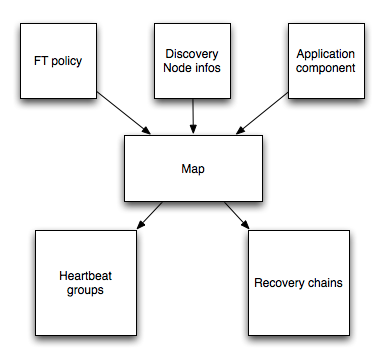
\includegraphics[width=\linewidth]{figures/mapping-ft}
\end{figure}

The figure~\ref{fig:mapping-ft} above shows the elements required in the
mapping process for a fault tolerant system.

Mapping is a process of converting a high level abstractions to low level
bytecode representation that will be deployed to the network.

The high level abstractions are the network node infos, application graph of
components and links, fault tolerance policy for components.

Mapper requires discovery of the network in terms of node infos, application
graph. In order to produce a fault tolerant system which satisfy fault
tolerance policy, mapper produces heartbeat groups and recovery chains
necessary to construct a fault tolerant system under the unique challenges of
heterogeneous sensor network modeled by sensor profile framework.

With heartbeat groups, a network of nodes will be able to detect a node failure
within the network efficiently, and able to reconfigure autonomously to reach
its stable state after the failure.

With recovery chains, the semantics of application will be persistent as
long as there is spare parts of components that could be recovered from
a node failure and still meet its application requirements.

\subsection{Heartbeat Groups}

Heartbeat is a heuristic to detect failure. Our work assume
a fail-stop model where sensor nodes fail by not sending messages for a period
of time. However, in a group of nodes, heartbeats needs to be arranged in such
a way that no failures could be left undetected. And thus Mapper will have to
determine the heartbeat arrangement, dependencies to ensure every sensor node
is monitored and will not fail without notice.

Heartbeat arrangement usually depends on the applications and sensor
arrangement~\cite{Gobriel2008}, thus most related work aim for a specific type of
application and sensor arrangement to simplify heartbeat arrangement, however
since application type and sensor arrangement in WuKong are not known until
deployment, therefore a new way to arrange heartbeat has to be devised.

In WuKong, applications are drawn on a canvas which consists of blocks that
gives the type of sensors or resources needed and lines which connects the
resources together in such a way that would satisfy the requirements. However,
arrange heartbeat based on the flow of the components is not desirable since
applications are not the immediate representation of the underlying network
topology such that some components could be mapped on the same node, and some
connected components could be mapped to nodes that are far away from each other
that require multiple hops to reach. Arrangement based on such high
abstractions would incur extra communication overhead by making a lot of nodes
as a relay for heartbeats.

The proposed solution will produce application agnostic arrangement and at
the same time be used in producing the arrangement of the components in the
network to reduce the communication overhead as much as possible.

The algorithm assumes that links are symmetrical and toplogy is stable after
making the arrangement.

Heartbeat groups are clustering of nodes
that are one hop distance to each other, in other words, fully connected. By
grouping nodes within one hop distance together, we significantly reduce the
possibility of heartbeat hopping which is a big factor in communication
overhead.

Heartbeat groups are determined by picking an anchor node by random in the
nodes, and then iterating through network of nodes to cluster nodes that are
meeting the criteria (one hop distance) and repeat again until all nodes are
exhausted. The function to determine topology of the network comes from the
hardware of the wireless radio specifications.

It is possible that due to some peculiar network topology that the
algorithm would produce single node group which itself could not be of any use.

If that happens, the algorithm will be rerun again. Since the anchor is picked
randomly from the remaining node list, the algorithm will not produce the same
result thus eliminating the problem.

Once the groups are formed, each group could employed many different heuristics
to connect such that any failure could be detected. One of the heuristics that
is used in this work is called daisy chain. Daisy chain makes every node
monitoring one other unique node in the network such that every node is
monitored with minimum communication overhead and an even communication load
for every node.

\subsection{Recovery chains}

When a component FT policy indicates a minimum redundancy level higher than
one, WuKong Master will map multiple eligible nodes to carry the WuObject
coresponding to the component and become the backups in case of a failure.

Since nodes could carry more than one component WuObject, and we assume
a heterogeneous network where it consists of nodes with different combinations
of capabilities, so for every comoponent WuObject there should be an ordered
list of nodes like a chain of command that when one of them failed, the next
one will be able to replace its place.

When a failure is detected, the detector is not necessarily carrying or knowing
what resources there are in the network at the given moment, and it would
produce an enormous of overhead to query for the resources in the network, so
with this ordered list of recovery, the information could be stored in advance
to prevent nodes having to do all the work over and over again whenever
a failure is detected. 

After mapping, the information of recovery is distributed accordingly based on
the heartbeat group results to ensure the integrity of recovery process such
that the detector will be able to recover broken links and update the nodes
that are affected.

The algorithm to produce the recovery chains is shown below, and it is
separated into several sections.

\subsubsection{Gather Candidates}

First it would have to sort and filter from the list of nodes discovered, which
are eligible to provide certain resources for components specified in the
application. Once it is sorted out, the algorithm will produce a dictionary of
component id as keys and list of node ids as values.

The algorithm requires node info of each node in the network. A node info
constitudes information such as a list of WuClasses and a list of WuObjects
that are used to help Master greatly in making an informed decision to gather
a list of eligible candidates for components.

\begin{algorithm}
\caption{Gather Eligible Candidates for Components}
\label{alg:recovery-chain}
\begin{algorithmic}
\Require A list $C$ of application component ids
\Require A list $I$ of node ids of the network
\Ensure A dictionary $D$ of component id as keys and list of node ids as values
\Function{isCapable}{$i, c$}
  \If{ComponentToWuClass($c$) in WuClasses($i$)}
    \State \Return \texttt{True}
  \Else
    \State \Return \texttt{False}
  \EndIf
\EndFunction
\For{Every $c$ in $C$}
  \For{Every $i$ in $I$}
    \If{isCapable($i$, $c$)}
      \State Add $i$ to $D$ under component id $c$ as key
    \EndIf
  \EndFor
\EndFor
\end{algorithmic}
\end{algorithm}

Function isCapable returns a boolean for whether the node is capable of
carrying the component

This algorithm will filter out and produce a list of eligible candidates for
every application component.

\subsubsection{Redundancy Level Enforcement}

Once the candidates has been gathered for every compoennt, here it will be
doing a check to enforce redundancy level policy to make sure all gathered
candidates are above the minimum redundancy level. If any of the candidates is
not satisfied, the deployment process will be terminated and the system will
send a warning to the users to inform of this situation.

\subsubsection{Sort Candidates}

It would be perfectly safe to deploy at this point with the unsorted candidates
for each component, but it will be running into a problem that could compromise
the operation of the system by unoptimized component arrangement. If the
components placement is unsorted, it is possible that unnecessary communication
would saturate the system thus compromising the health of the application. On
the other hand, if the placement is carefully analyzed, the impact of the
overhead could be minimized to certain degrees such that the system could run
when deployed.

\begin{algorithm}
\caption{Build histogram of the nodes appear in candidate list}
\label{alg:build-histogram}
\begin{algorithmic}
\Require A dictionary $D$ of unsorted recovery chains of every component
\Ensure A dictionary $H$ of node ids and number of occurrances
\For{Every $c$ in $C$}
  \For{Every $n$ in $D[c]$}
    \If{$n$ not in $H$}
      \State $H[n] = 1$
    \Else
      \State $H[n] = H[n] + 1$
    \EndIf
  \EndFor
\EndFor
\end{algorithmic}
\end{algorithm}

\begin{algorithm}
\caption{Sort Recovery chains}
\label{alg:sort-recovery-chain}
\begin{algorithmic}
\Require A list $C$ of components
\Require A dictionary $D$ of unsorted recovery chains of every component
\Require A histogram $H$ of all nodes
\Ensure A dictionary $D$ of sorted recovery chains of every component
\For{Every $c$ in $C$}
  \State Sort $D[c]$, and use $H$ as keys in decending order
\EndFor
\end{algorithmic}
\end{algorithm}

By sorting based on the occurrances of node as candidates, the nodes with
highest scores will be hosting a lot more components thus reducing external
communications within the system especially for the case when WuObjects are
linked but are placed in separate nodes.

\subsection{Determine Heartbeat Group Period}

Once the placement and ordering for the components in forms of recover chains
are decided, the heartbeat interval for heartbeat groups could be deteremined.
Since heartbeat groups could have multiple components, the group heartbeat
period is half of the minimum maximum reaction time policy of the components.

Our system assumes a fail-stop model where nodes are suspected dead when it
does not send out messages, but to compensate possible deviation in
communication latency, a failure is detected when the node does not send
a heartbeat message within two normal heartbeat periods. Thus the heartbeat
period is half of the reaction time.

\begin{algorithm}
\caption{Determine Group Heartbeat Period}
\label{alg:determine-group-heartbeat-period}
\begin{algorithmic}
\Require A list of heartbeat groups $H$
\Ensure A list of heartbeat groups with heartbeat periods
\For{Every heartbeat group $g$ in $H$}
  \For{Every component Component($n$ in $g$)}
    \State Find the lowest minimum reaction time
    \State Divided in hald and assign the period to group $g$
  \EndFor
\EndFor
\end{algorithmic}
\end{algorithm}

Since all nodes within the heartbeat group is compared against, so only the
lowest time will be picked.

\section{Information Distribution}

After mapping and produced heartbeat groups for the network and recovery chains
for the components, WuKong would have to generate and assignment information
appropriated to every node to support fault tolerance.

Every node will have information pertain to the list below:

\begin{enumerate}
\item Recovery chains for the mapped components
\item List of nodes of the heartbeat group it is in
\item The recovery chains of the node it will monitor based on
the heartbeat arrangement
\item The application links of the components assigned to the node it will
monitor based on the heartbeat arrangement
\item Heartbeat period of the group it is in
\end{enumerate}

\section{Application generation}

WuKong runs a JVM on every node in the network, the VM provides services for
the application program in Java to access lower parts of the resources.
This section will introduce the list of newly added interfaces and resources to
support and enable fault tolerance for the application.

\begin{enumerate}
\item component instance id to WuObject address map
\item heartbeat groups member list
\item heartbeat group period list
\end{enumerate}

\section{Wireless Deployment}

The rest of the deployment is the same as the deployment described in the
background work for WuKong, where after it generates the Java code, it compiles
down to lower bytecode representation and send it to every node wirelessly. The
nodes will be reprogrammed by taking the code and reload in their flash memory.


%%%%%% end of mapper %%%%%%
%%%%%% end of mapper %%%%%%


\section{Fault Tolerance System}

% begin comment
\begin{comment}
\subsection{Agent architecture}

This section will first go into details of how applications in a form of an
abstract graph are being managed in a distributed system after being compiled 
and transformed into lower bytecode representation, then I will further discuss 
how the agent architecture on every node collaborate to for the basic unit of
redundancy in the application to detect sensor failures, diagnosis the failure,
and finally recover from failure.

\subsection{Autonomous Systems}

Sensor networks composed of a large number of diverse subsystems. Subsystems
intertwined with complex relationships that prohibit human intervention.
Subsystems such as deployment, operation, reconfiguration, maintenance must be
automated.

The inability, passiveness to errors makes the past systems unable to deal with
perturbations, or unpredictable changes in the environment. Such systems know
a limited amount of patterns and trigger predefined actions when they encounter
these patterns. In order to make system adapt to new environment in a way
similar to biological systems, they need to react to events as a whole in
real-time.

\subsection{Distributed agents}

As our system consists of complex elements and subsystems mingled together, an
appropriate way to handle complex behaviors in decentralized systems is to
based it on a society of agents.~\cite{Minar1999}
\end{comment}
% end comment

\subsection{Towards Failure Detection}

As we mentioned earlier why sensor system has to evolve to adapt to crutial,
ever changing environment, one of the first things a system could achieve that
goal is to detect failures autonomously.

\subsubsection{Heartbeat}

A failure in distributed system could come from different causes. Some nodes
might fail because of software bugs; some nodes might appear to fail because of
poor wireless link quality. One of the biggest challenges in distributed
systems is to be able to detect failures when it occurs accurately.

In distributed system, nodes could fail. In order to be consistent, we model
failure by whether a node send messages within predefined period or not. It is
called a fail-stop failure model.

Heartbeats are messages sent by individual nodes periodically to indicate to
the monitoring nodes its health.

Figure~\ref{} illustrates some nodes sending heartbeats that detects
a failure when a number of expected consecutive heartbeats have not been
received.

In our model, a node is considered dead when it has not been sending heartbeats
for more than 2 timeout periods.

% figures to illustrate how heartbeat works?

\subsubsection{Decentralized Detection}
% daisy chain

In a network of nodes, the arrangement of heartbeats has to be addressed to
have full coverage of the network such that every node is monitored by another
node which is also monitored by another node and is decided during the mapping
phase mentioned in the previous section.

Centralized detection makes one special node to monitor every node in the
network by making them sending heartbeats to it. The arhictecture has several
weak points where it requries extra resources to monitor, and since the
monitoring node cannot be replaced when failed, the system will have single
point of failure. In addition to that, the average communication overhead for
the monitoring node will be very high and saturated since all the traffic goes
towards one place and thus the system performance will deteriorate.

% introduction to heartbeat network

A heartbeat can only monitor one node at a time, so in a network of nodes, we
need a heartbeat network. The structure of heartbeat communication pattern
highly depends on the underlying network assumption and infrastructure of the
application. To produce the most efficient network with the least connections,
  heartbeat network has to satisfy two properties.

\begin{enumerate}
\item Every node has to monitor at least one node other than itself
\item Every node can only has one node monitoring itself
\end{enumerate}

% why daisy chain, what's the benefits? How does it affect other fault
% tolerance policies?

A heartbeat network in the form of a daisy chain is one of the networks that
satisfy both properties as shown in~\ref{fig:daisy-chain}. Every daisy chain
heartbeat network monitors all nodes in the group, given by the properties that
every node has to monitor at least one node and every node can only have one
node monitor itself. So if there is n nodes, there can be at most n nodes being
monitored, every monitoring node can only monitor one node, every node can only
monitor node that others have not, thus every node is monitored by only one
unique node. Thus this daisy chain guarantees every failure can be detected.

\begin{figure}[h!]
\label{fig:daisy-chain}
\caption{Daisy Chain of heartbeats}
\centering
    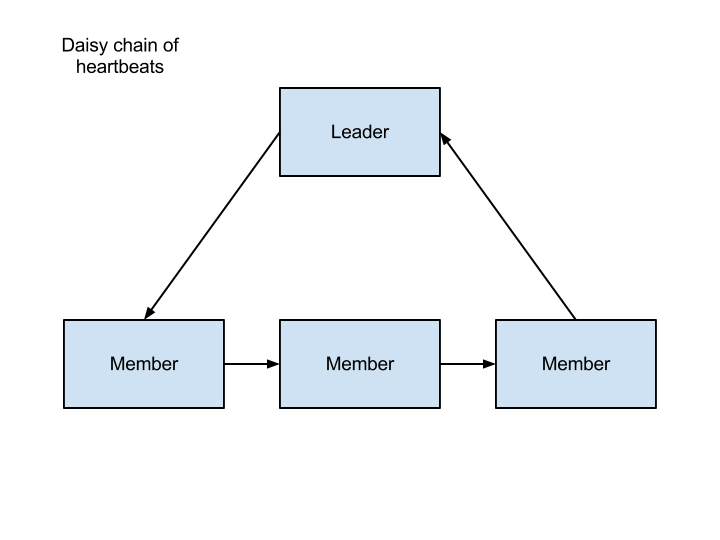
\includegraphics[width=\linewidth]{figures/daisy-chain}
\end{figure}

\paragraph{Message complexity}

Every heartbeat takes one message to send from one to another. As of current,
we assume every heartbeat is sent using unicast, and there is no ACK for
heartbeat messages. The message complexity for standard one-hop star
network takes about
O(2n-2) messages since the leader sends n-1 to every member and every
member would also has to send a message back to leader, that comes to
double of the single traversal from leader to other members.

The message complexity for the daisy loop takes about $O(n)$ messages for
a group, because every member only sends one heartbeat to one other member at
a time including the leader.

\subsubsection{Heartbeat Group Recovery}

When a node failed and stopped sending heartbeats, the existing network of
heartbeat needs to recover its arrangement to handle the next error. If we are
given a network of nodes with heartbeat arranged like in
Figure~\ref{fig:daisy-chain}, when the leader failed and is picked up by the
member, the member that is monitoring the leader will notify the member that is
monitored by the old leader to redirect its heartbeat to itself instead so the
loop hole is closed. Algorithm~\ref{alg:recover-heartbeat-group} described what
happened when a node detects a failure.

\begin{algorithm}
\caption{Recover Heartbeat Group (at detected node)}
\label{alg:recover-heartbeat-group}
\begin{algorithmic}
\Require A list of node ids $G$ of the heartbeat group it is in
\Require Failed node id $f$
\Ensure Update list of node ids $G$ of the heartbeat group in other members
\State Remove failure node id $f$ from local Heartbeat Group $G$
\State Update the new node id to monitor which is the node before its id in the
list
\For{Every $n$ in $G$}
  \State Send message to $n$ to upload their local heartbeat group and update
  their monitoring node id
\EndFor
\end{algorithmic}
\end{algorithm}

The algorithm requires synchronization among all heartbeat group members since
if it only updates the affected nodes then after two specific node failures in
such order that the node will not be able to recover from failure. It is
illustrated in Figure~\ref{fig:recovery-heartbeat-group-need-synchronization}

\begin{figure}[h!]
\label{fig:recovery-heartbeat-group-need-synchronization}
\caption{Heartbeat group cannot recover}
\centering
    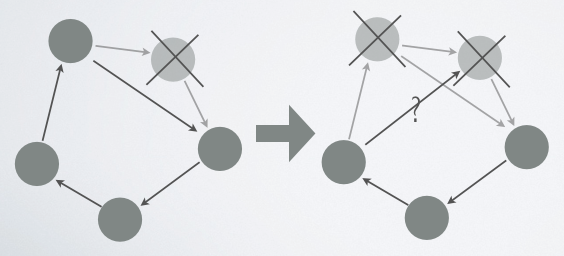
\includegraphics[width=\linewidth]{figures/recovery-heartbeat-group-need-synchronization}
\end{figure}

In the first failure, the previous node could update its local list point to
the alive node to monitor, but if the node fails, the next node will not point
to the alive node to monitor.

%%% end of failure detection %%%

\subsection{Failure Recovery}

% mention the needs for at least one substitude, and how the candidate is
% selected

Due to the nature of the network that will have lots of recovery chains for
several application components on different or same nodes, when a node detects
failure in a node, the detector will initiate a failure recovery protocol to
recover the affected component recovery chains and application links for
nodes hosting connected components.

The detector of node failure will determine the WuObjects running on node, to
update recovery chains in the network, and to determine nodes that host
connected WuObjects. For example, if node A runs WuObject 1, and when WuObject
2 which is hosted on node B is connected, node B is the node hosting the
  connected WuObjects.

\subsubsection{Recover Chains}

The algorithm~\ref{alg:recover-recovery-chains} describes how the node detected
the failure will have to update recovery chains of all nodes that is hosted on
the dead node.

\begin{algorithm}
\caption{Recover Recovery Chains (at detected node)}
\label{alg:recover-recovery-chains}
\begin{algorithmic}
\Require A list of components $C$ of the failure node
\Require Failed node id $f$
\Ensure Update all host hosting component in $C$ their local recovery chain
lists
\State Remove failure node id $f$ from all local recovery chains of component in $C$
\State Update nodes of their recovery chains in the components in $C$
\end{algorithmic}
\end{algorithm}

\subsubsection{Connected Nodes}

The algorithm~\ref{alg:update-application-links} describes how the node detected
the failure will have to update application links of all nodes that is
connected to components on the dead node.

\begin{algorithm}
\caption{Update Application Links (at detected node)}
\label{alg:update-application-links}
\begin{algorithmic}
\Require A list of components $C$ of the failure node
\Require A list of links of components $L$ of the failure node
\Require Failed node id $f$
\Ensure Update all local links in $L$ to point to next alive node for the component
with the dead node
\State Update links of nodes that host components that is connected to the
original component with the dead node
\end{algorithmic}
\end{algorithm}
